\documentclass{article}

\usepackage[final]{../neurips_2019_230}
\usepackage[utf8]{inputenc}
\usepackage[T1]{fontenc}
\usepackage{hyperref}
\usepackage{url}
\usepackage{booktabs}
\usepackage{amsfonts}
\usepackage{nicefrac}
\usepackage{microtype}
\usepackage{graphicx}
\usepackage{xcolor}
\usepackage{lipsum}
\usepackage{lipsum}
\usepackage{graphicx}
\usepackage{subcaption}

%\usepackage[margin=0.5in]{geometry}
%\setlength{\textwidth}{7.5in}   % Adjust text width
%\setlength{\textheight}{10in}   % Adjust text height
%\setlength{\oddsidemargin}{-0.5in} % Adjust left margin
%\setlength{\evensidemargin}{-0.5in} % Adjust right margin
%\setlength{\topmargin}{0in} % Adjust top margin
%\setlength{\headheight}{3pt}  % Adjust header height (if needed)

%\usepackage{showframe}

\newcommand{\note}[1]{\textcolor{blue}{{#1}}}

\title{Mathematical Problem Solving with Language Models (Natural Language)
  %Title of your project \\
  %\vspace{1em}
  %\small{\normalfont Stanford CS229 Project}  % Select one and delete the other
}

\author{
  Yacine Dolivet\\
  \texttt{yacine@stanford.edu} \\
  \And
  Stephen Ge\\
  \texttt{scge@stanford.edu} \\
   \And
  Sasha Kuznetsov\\
  \texttt{skz@stanford.edu} \\
  % Examples of more authors
%   \And
%   Name \\
%   Department of Computer Science \\
%   Stanford University \\
%   \texttt{name@stanford.edu} \\
%   \And
%   Name \\
%   Department of Computer Science \\
%   Stanford University \\
%   \texttt{name@stanford.edu}
}

\begin{document}

\maketitle

%\begin{abstract}
%The abstract is optional, depending on your available space. It should consist of 1 paragraph consisting of the motivation for your paper and a high-level explanation of the methodology you used/results obtained.
%\end{abstract}


% {\color{red} This template does not contain the full instruction set for this assignment; please refer back to the milestone instructions PDF.}

\section{Introduction}
We evaluate and aim to improve the mathematical reasoning abilities of small (<10B parameters) language models (LMs). This is interesting because LLMs can produce text which seems logically and reasonably sound but often contains mathematical or reasoning errors. The inputs to our evaluations are various open source language models such as Llama 3 \citep{dubey}, OpenMathInstruct-2 \citep{toshniwal}, Phi-3.5 \citep{abdin}, and datasets such as GSM8K \citep{cobbe}, GSM-IC \citep{shi}, and our own synthetic datasets.

We investigate methods to detect the presence of irrelevant information in math problems via training linear probes (\citep{alain} \citep{hewitt}) and direct prompting. We propose a two-stage pipeline to recover performance drop from distractors in math problems similar to corresponding strategies in computer vision\footnote{See YOLO \citep{redmon}, and SK patent \citep{US20230091374A1}}.

\section{Related Work}
A series of techniques have been developed to improve the reasoning capabilities of large language models, particularly in mathematical problem solving. These include Chain-of-Thought prompting \citep{wei}, self-consistency decoding strategy \citep{wang}, process supervision \citep{lightman}, and conversion of the math problem reasoning task into one of generating a Python program that returns a correct answer \citep{chowdhery}.

There is also a collection of related work in the adversarial or challenge dataset direction, demonstrating pitfalls or difficulties with eliciting correct reasoning from large language. GSM-Plus \citep{li} adds variations and distractors onto the original GSM8K dataset. Irrelevant context in particular is studied in \citep{shi}. \citep{mirzadeh} conduct a large scale study across numerous models using new GSM-Symbolic and GSM-NoOp datasets changing symbolic values and adding additional clauses.

\section{Dataset and Features}

The original GSM8K data from \citep{cobbe} contains 7.5k training and 1k test "high quality linguistically diverse grade school math world problems". We use the subset of "distraction insertion" of GSM-Plus from \citep{li} along with their associated seed questions from the original GSM8K data set as our holdout test set for final evaluations. We refer to this subset as GSM-Plus-Distractor.

For the purposes of training the classifiers, we synthetically generate additional distractor containing samples from each of the 7.5k original GSM8k training set problems. We use GPT-4o and a similar question variation generating prompt as in \citep{li}. As our synthetic data was purely for the purposes of training a probing classifier, we did not engage in further refinement via human annotators or otherwise for solvability criteria.

The original 7.5k word problems from GSK8K along with our additional distractor insertion problems were passed into the Llama3.1-8B-Instruct language model, from where we obtained the activations at each of the layers. For each layer of the language model, we thus had 15k examples, half of which had the True or positive label for containing a distractor (the synthetic examples we generated), and half of which had the False or negative label (the original GSM8K) problems. Each example produced a pooled tensor of 4096 features, the hidden-model dimension of Llama-3.1-8B, along with a boolean label of whether the problem text contained irrelevant information. We ran various pooling methods (mean, variance, final token) to go from raw activations (of dimension sequence-length x hidden-dimension) to the examples to be passed into the classifier.

We also initially evaluated the GSM-IC \citep{shi} "irrelevant context" dataset. However both the Llama-3.1-8B-Instruct and OpenMathInstruct2 models had unexpectedly high performance, leading us to search for alternative challenge datasets. See Table~\ref{tab:gsm_ic_metrics} in the Appendix for GSM-IC evaluation results.

\section{Methods}

\subsection{Pipeline}

We propose a pipeline which includes a "gating" classifier model, which classifies a word problem as likely containing distracting information. If it does, we attempt to modify the prompt to improve performance. Such a "gating" model can avoid confusing the downstream LLM because we only hint or attempt to remove the distracting information if we believe it exists, or it can improve efficiency since an attempt to remove distracting information will not always be performed. This draws inspiration from computer vision applications \citep{US20230091374A1}, where "gating" models control heavier, downstream models. 

\begin{figure}[h!]
    \centering
    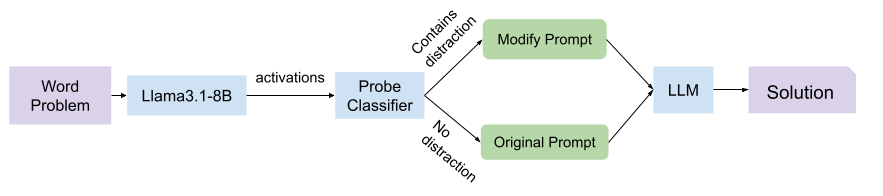
\includegraphics[scale=0.4]{tex/finalreport230/pipeline_diagram_cropped.png}
    \caption{Pipeline which uses classification result to modify prompt if it likely contains distracting information}
    \label{fig:pipeline_diagram}
\end{figure}

\subsection{Detecting Irrelevant Clauses Via Probing}
We attempt to train a classifier which, by probing layers of the LLM, can determine from the latent activations whether the problem may include irrelevant information that is confusing the LLM. 

\subsubsection{Probe Architecture}

\begin{figure}[h!]
    \centering
    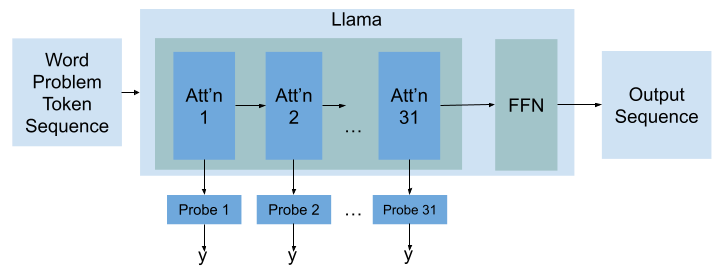
\includegraphics[width=0.7\linewidth]{tex/finalreport230/probe_diagram_cropped-2.png}
    \caption{Probing Architecture}
    \label{fig:variance_pooling_training}
\end{figure}

We trained a probe on each of the 31 attention layers of Llama3.1-8b-Instruct, skipping the first embedding layer. Each attention layer has a hidden dimension of 4096. With a maximum sequence length choice of 512 tokens, this produces an activation tensor of 512x4096.

To reduce the model complexity, we explored various techniques to pool over the sequence, namely:

\begin{itemize}
    \item Last token pooling
    \item Mean Pooling
    \item Variance Pooling 
    % \item Energy Weighted Pooling
\end{itemize}

Each of these techniques reduced the probe input size to 4096 dimensions. 

We explored both simple linear probes as well as complex 2-hidden layer probes. 

Probes were trained on synthetic data, attempting to classify each word problem as either containing or not containing irrelevant information, optimizing for cross entropy loss. 

\subsubsection{Sequence Pooling Techniques}

Detecting irrelevant information in a sequence may require different pooling methods than those commonly used for tasks like sentiment analysis. In sentiment analysis, mean pooling or attention-weighted pooling often suffice because the overall sentiment can be captured by averaging token embeddings or focusing on sentiment-heavy words. However, identifying irrelevant or outlier information requires pooling functions that are sensitive to anomalies or deviations within the sequence.

The intuition behind Variance Pooling being that embeddings of the potential irrelevant clause could look different from the average embeddings of the sequence. 

Other methods of statistical pooling are described in \cite{Zamanzadeh_Darban_2024}.

\subsubsection{Base LLM Choice}
We experimented with training probes on both the Llama3.1-8B-Instruct and its fine-tuned Openmath variant. However, because the Openmath variant is already finetuned on gsm8k, which was one of our evaluation sets, we considered that this may not be a fair evaluation.  

\subsubsection{Linear vs Complex Probes}
We experimented with both linear and complex probes. We found that linear probes were sufficient for the classification task, and complex neural network probes had more of a tendency to overfit to the training data. 

\subsubsection{Caching Activations}
To increase training and iteration speed, we only generate and save layer activations once for each pooling technique, then we train each probe on the cached activations. This works well because we are not fine-tuning the Lllama model itself, so the activations do not change while training probes. 
 
% \subsection{Synthetic Python Program Generation To Improve Reasoning Ability}

% We aim to create a dataset of word problems from a simple python function involving only basic arithmetic operations and prompt a frontier language model to generate grade school math problems corresponding to the function. For example, from the function 
% \begin{center}
% \begin{verbatim}
%   def mod(a,b,c,d):
%     answer = a * 90/100 - b * c + a * b * c + d
% \end{verbatim}
% \end{center}
% the following problem was generated 
% \begin{verbatim}
% Problem 1
% [GSP]  
% A museum sells an entrance ticket for $50. There is a 10% discount for
% online purchases. A visitor buys 2 art guides priced at $15 each. The 
% museum has a special promotion that deducts the total cost of the art
% guides from the ticket price. Additionally, a processing fee of $10 is
% added for buying tickets online. What is the total cost for the visitor?  
% [GSP] 
% \end{verbatim}

% Then we can create variations of the this word problem which map to the same python function required to solve it.

% We then feed these word problems into an LLM and compare the python function it generates against the ground truth function. Our intuition is that it will be easier to evaluate the correctness of the solution by evaluating the equivalence of the generating python function, and the generated python function. 

% As part of this exploration, we also aim to see if we can train probing models, which take in layer activations from the LLM, to determine if two python functions are equivalent, the motivation being that the hidden activations may contain semantic information about the python programs which capture equivalence. 

\subsection{Instruction Prompting the Language Model to Ignore Distractor}

For irrelevant context, we attempt to prompt the language model to ignore any irrelevant information present in the problem description \citep{shi}. We evaluate both a soft version (IC Prompt) \textit{"Solve the following math problem. Feel free to ignore irrelevant information given in the questions."} and also an explicit version (IC Prompt Explicit) \textit{"The following math problem contains irrelevant information. Ignore the irrelevant information and solve the math problem."} that can be used as the second stage of a pipeline depending on the probe classification output. We compare against \textit{"Solve the following math problem."} as a baseline (Default) in Table~\ref{tab:prompt_metrics}. Note that all prompts have \textit{"Make sure to put the answer (and only answer) inside \textbackslash boxed\{\}."} post-pended for consistency in evaluation processing.

We evaluated all variations of model, dataset, and prompt with the NeMo-Skills framework \citep{toshniwal}.


\section{Experiments / Results / Discussion}



\subsection{Probe Classifiers}
We trained linear probe classifiers on all 31 attention layers of Llama3.1-8B-Instruct on our synthethically augmented dataset. Then, we evaluated, by layer, each trained classifier on the GSM-IC distracted set, which was not used for training. We evaluated using both the classification threshold which maximized the F1 score on the validation set, and an apriori classification threshold of 0.5 probability. The code for this exploration can be found at \citep{skzv2024mathlm}, with evaluation results in Table~\ref{tab:classifier_metrics}.

% To prepare for training probes on the layer activations to detect irrelevant clauses and function equivalence, we are first training simple sentiment classifiers on LlaMa3.1-8B layer activations, using examples from the Glue-SST2 dataset \citep{wang2018glue}. We observed that a linear probe does not seem expressive enough for this task, so we are experimenting with small FC-ReLU-FC NNs that consume these layer activations. The code for this exploration can be found at \citep{skzv2024mathlm} and training results can be seen below. Since the plots show improving validation accuracy - without overfitting -  we have increasing confidence this model may be expressive enough to learn the tasks we are interested in. 

\subsubsection{Probing Performance by Layer}
We observed that, regardless of sequence pooling choice, performance - as measured by classifier AUC - increased with layer depth. This strong relationship is visible in Figure~\ref{fig:training_test_auc_vs_layer}. Our intuition is that later layers are successfully capturing higher abstract information, which for our task includes the presence of irrelevant or distracting information.

\subsubsection{Sequence Pooling Choice}
We found that our sequence pooling choices were comparable. We observed that variance pooling maximized the F1 score. Refer to Table~\ref{tab:classifier_metrics} for a detailed evaluation. 

\subsubsection{Classification Threshold Choice}
We attempted to choose an optimal classification threshold by using the threshold that optimizes the F1 score on the validation set. However, this performed worse on the test than just using an apriori assumed classification threshold of $p=0.5$. See Figure~\ref{fig:confusion_matrices}, which shows how the apriori classification threshold confuses the model less than the validation set F1-score maximizing threshold. Also see Figure~\ref{fig:roc_curves}, which shows that different classification thresholds (in logit space) maximize performance between the validation and test sets\footnote{Since we have effectively a mismatched data set, in order to rectify this in a future experiment, split our GSM-IC distracted set intro train and validation set and keep some portion for the train set to make distributions more comparable}

\begin{figure}[h!]
    \centering
    \begin{subfigure}[b]{0.48\linewidth}
        \centering
        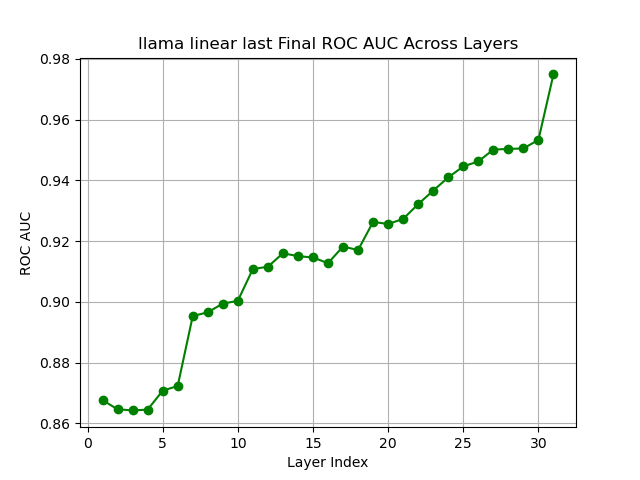
\includegraphics[width=\linewidth]{tex/finalreport230/last_pooling_train_auc_vs_layer.png}
        \caption{AUC vs layer on validation set}
        \label{fig:last_pooling_train_auc_vs_layer}
    \end{subfigure}
    \hfill
    \begin{subfigure}[b]{0.48\linewidth}
        \centering
        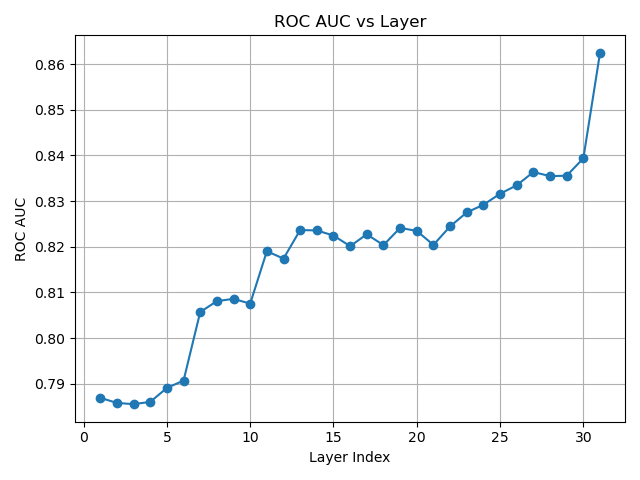
\includegraphics[width=\linewidth]{tex/finalreport230/last_pooling_test_auc_vs_layer.png}
        \caption{AUC vs layer on test set}
        \label{fig:last_pooling_test_auc_vs_layer}
    \end{subfigure}
    \caption{AUC vs layer on validation and test sets for last token pooling. They exhibit similar trends where later layers are more useful for the classification task, but the AUC on the test is lower than the validation set. A similar relationship was observed for every pooling choice.}
    \label{fig:training_test_auc_vs_layer}
\end{figure}

\begin{figure}[h!]
    \centering
    \begin{subfigure}[b]{0.48\linewidth}
        \centering
        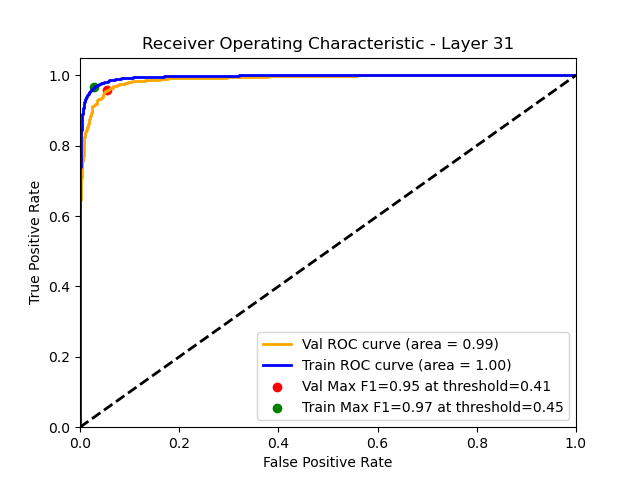
\includegraphics[width=\linewidth]{tex/finalreport230/variance_roc_curve_layer_31_training.png}
        \caption{Layer 31 variance pooling ROC curve on training/validation}
        \label{fig:train_roc_curve}
    \end{subfigure}
    \hfill
    \begin{subfigure}[b]{0.48\linewidth}
        \centering
        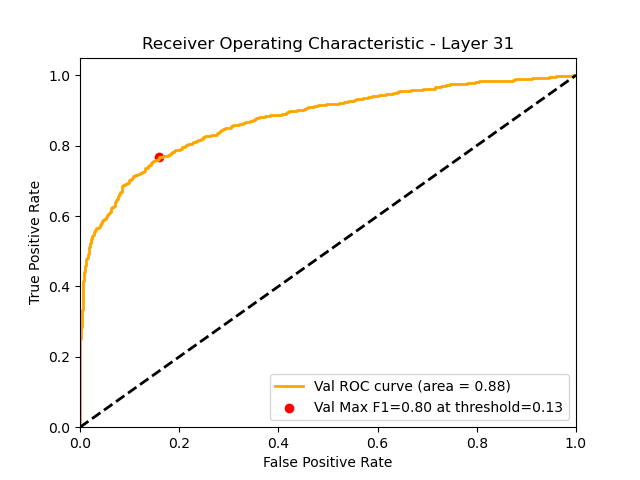
\includegraphics[width=\linewidth]{tex/finalreport230/variance_roc_curve_layer_31_test.png}
        \caption{Layer 31 variance pooling ROC curve on training/validation}
        \label{fig:test_roc_curve}
    \end{subfigure}
    \caption{Final attention layer ROC curves on train/val dataset (synthetically generated) and test dataset (GSM-IC distracted)}
    \label{fig:roc_curves}
\end{figure}

\begin{figure}[h!]
    \centering
    \begin{subfigure}[b]{0.48\linewidth}
        \centering
        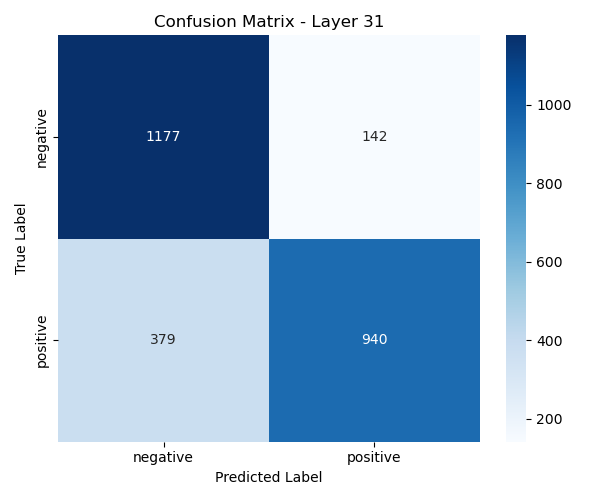
\includegraphics[width=0.8\linewidth]{tex/finalreport230/variance_confusion_matrix_layer_31_f1_max_threshold.png}
        \caption{Layer 31 confusion matrix on test set with validation F1-score maximizing threshold}
        \label{fig:cm_f1}
    \end{subfigure}
    \hfill
    \begin{subfigure}[b]{0.48\linewidth}
        \centering
        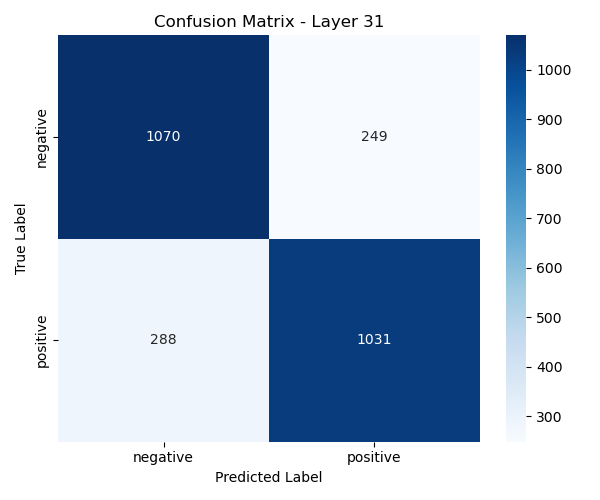
\includegraphics[width=0.8\linewidth]{tex/finalreport230/confusion_matrix_layer_31_apriori_threshold.png}
        \caption{Layer 31 confusion matrix on test set with apriori assumed p=0.5 classification threshold}
        \label{fig:cm_apriori}
    \end{subfigure}
    \caption{Confusion matrices showing how using apriori assumed p=0.5 classification threshold confuses the model less than using the threshold that maximized the F1 score on the validation set}
    \label{fig:confusion_matrices}
\end{figure}

% \begin{figure}[h!]
%     \centering
%     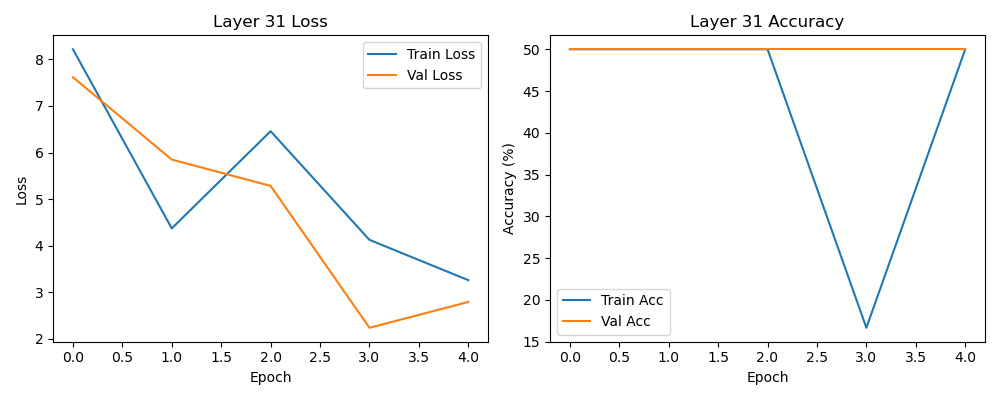
\includegraphics[width=\linewidth]{layer_31.png} % Adjust the width as needed
%     \caption{Probe training/validation loss and accuracy on a sentiment classification task by consuming activations from the 31st layer of Llama3.1-8B. We aim to extend this approach to detect irrelevant clauses and functional equivalence between python programs.}
%     \label{fig:layer31}
% \end{figure}

\begin{table}[h!]
    \centering
    \begin{tabular}{l c c c c c}
        \toprule
        \textbf{Classifier Variant} & \textbf{Precision} & \textbf{Recall} & \textbf{FPR} & \textbf{TPR} & \textbf{F1} \\
        \midrule
        Last token pooling - layer31 - 0.5 threshold & 0.83 & 0.71 & 0.15 & 0.71 & 0.76\\
        Last token pooling - layer31 - val-f1-max-threshold & 0.91 & 0.56 & 0.05 & 0.56 & 0.69\\
        Mean pooling - layer31 - 0.5 threshold & 0.79 & 0.77 & 0.21 & 0.77 & 0.78 \\
        Mean pooling - layer31 - val-f1-max-threshold & 0.88 & 0.63 & 0.09 & 0.64 & 0.74 \\
        \textbf{Variance pooling - layer31 - 0.5 threshold} & \textbf{0.81} & \textbf{0.78} & \textbf{0.19} & \textbf{0.78} & \textbf{0.79} \\
        Variance pooling - layer31 - val-f1-max-threshold & 0.87 & 0.71 & 0.11 & 0.71 & 0.78 \\
        % Energy pooling - 0.5 threshold & & & & & \\
        % Energy pooling - train-f1-max-threshold & & & & & \\
        \bottomrule
    \end{tabular}
    \caption{Comparison of pooling methods with precision, recall, FPR, TPR, and F1 metrics.}
    \label{tab:classifier_metrics}
\end{table}

\subsection{Instruction Prompting Performance}
We evaluated Llama-3.1-8B-Instruct and OpenMath2-Llama3.1-8B on the GSM8K and GSM-Plus-Distractor test sets with various prompting methods (Table~\ref{tab:prompt_metrics}). We see that OpenMath2 performance drops from 91\% to 78\% due to the distractor inclusion, but overall performance is essentially unaffected by prompt variation. This could be due to OpenMath being fine tuned from Llama3.1-8B-Base on large amounts of math problem data, while not being instruction tuned on general data. Llama-3.1-8B-Instruct experiences a performance drop of 13\% (82.5\% to 69.5\%) from the distractor insertion. We see that instructing with irrelevant context prompts recovers about 30\% (4\% out of 13\%) of the performance drop, with the explicit prompt also negatively affecting GSM8K performance. This gives the potential for the classifier to boost performance of an overall pipeline.

\begin{table}[h!]
    \centering
    \begin{tabular}{l c c c c c}
        \toprule
        \textbf{Model - Dataset} & \textbf{Default} & \textbf{IC Prompt} & \textbf{IC Prompt Explicit} \\
        \midrule
        Llama3.1-8B - GSM8K & 82.56 & 82.94 &  80.74   \\
        Llama3.1-8B - GSM-Plus-Distractor & 69.52 & 73.69 & 73.16 \\
        OpenMath2-Llama3.1-8B - GSM8K & 90.83 & 90.98 & 91.21  \\
        OpenMath2-Llama3.1-8B - GSM-Plus-Distractor & 77.79 & 77.86 & 78.47 \\
        \bottomrule
    \end{tabular}
    \caption{Comparison of irrelevant context instruction on various language models and datasets}
    \label{tab:prompt_metrics}
\end{table}

\subsection{Combining Classifier and Prompting}
The classifier and prompting can be combined into a two stage pipeline to boost solving performance on the combined GSM8K and GSM-Plus-Datasets. We propose given a test problem that may or may not have irrelevant information, first use the trained probing classifier to detect the presence of a distractor. If the classifier returns false, we then use the Default prompt. If the classifier returns true, we use the explicit IC Prompt affirming the presence and instructing to ignore distractor in solving. Given a true positive rate of 87\% for the first stage classifier, we estimate a 26\% (87\% times 30\%) recovery of the performance drop from distractor insertion for the two stage pipeline combining the trained classifier with instruction prompting on explicit presence of irrelevant information.

\section{Future Work}
In the future we plan to combine the classifier with prompting to perform a full-end-to-end evaluation, perhaps with a more advanced model for problem solving while retaining a small lightweight model for classification. 

\section{Contributions}
YD and SK led infrastruture exploration, in particular compute platforms and inference, evaluation, and training pipeline (NeMo Skills). SK is exploring training layer probes for perturbation and functional equivalence detection. YD is exploring the functional equivalence direction.  SG explored research directions, carried out initial experiments with GSM-IC on recent small LMs, and is exploring further perturbations.

We benefited from conversations with Neil Band, Ryan Chi, JB Jong Beom Lim, and Kamyar Salahi.

\bibliographystyle{plain}
\bibliography{references}

\section{Appendices} 

\begin{figure}[h!]
    \centering
    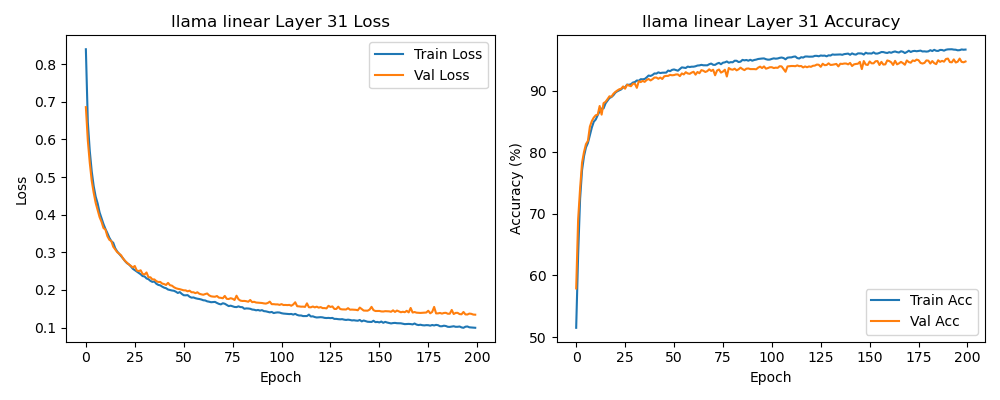
\includegraphics[width=\linewidth]{tex/finalreport230/llama_variance_pooling_training_plot.png}
    \caption{Training linear probe with variance pooling}
    \label{fig:variance_pooling_training}
\end{figure}

\begin{table}[hbp]
    \centering
    \begin{tabular}{l c c c c c}
        \toprule
        \textbf{Model} & \textbf{GSM-IC-2Step} & \textbf{GSM-IC-Mstep}  \\
        \midrule
        Llama3.1-8B & 95.06 & 91.69   \\
        OpenMath2-Llama3.1-8B & 96.48 & 97.16   \\
        Phi3-Mini & 44.07 & 44.07 \\
        \bottomrule
    \end{tabular}
    \caption{Various small language model performances on GSM-IC dataset, where a score of 100 is recovering original performance without any distraction}
    \label{tab:gsm_ic_metrics}
\end{table}
\end{document}
